\documentclass[final]{hcmut-report}
\usepackage{fontspec}
\usepackage{tabularx,microtype,xurl,amsmath}
\setlength{\parindent}{0pt}
\setlength{\parskip}{4pt}
\setstretch{1.08}
\setlength{\textfloatsep}{10pt plus 2pt minus 2pt}
\setlength{\headheight}{44.3pt}
\setlength{\emergencystretch}{2em}
\setcounter{tocdepth}{1}
\newcolumntype{Y}{>{\raggedright\arraybackslash}X}
\newfontface\VietnameseNames{lmroman12-regular.otf}
\newcommand{\vn}[1]{{\VietnameseNames #1}}
\newcommand{\code}[1]{\texttt{\detokenize{#1}}}
\newcommand{\source}[2]{\href{#1}{#2}}
\newcommand{\stage}[1]{\fcolorbox{blue!35!black}{blue!4}{\strut #1}}
\deptname{Faculty of Computer Science and Engineering}
\coursename{Deep Learning and Its Applications (CO3133)}
\reporttype{Assignment 3 M2 Draft Report}
\title{Product Type Classification with Amazon Berkeley Objects}
\advisor{Dr. Le Thanh Sach}
\groupname{Tiki-taka}
\logofile{hcmut.png}
\hypersetup{pdftitle={Tiki-taka Assignment 3 M2 Draft Report},pdfauthor={Tiki-taka}}

\newcommand{\ABOSplitRows}{%
TABLE & 332 & 71 & 71 & 474\\%
CHAIR & 894 & 192 & 192 & 1,278\\%
LAMP & 256 & 55 & 55 & 366\\%
STOOL\_SEATING & 229 & 49 & 49 & 327\\%
LIGHT\_FIXTURE & 282 & 60 & 60 & 402\\%
SOFA & 510 & 109 & 109 & 728\\%
GROCERY & 1,256 & 269 & 269 & 1,794\\%
SHOES & 445 & 96 & 95 & 636\\%
RUG & 530 & 114 & 113 & 757\\%
WALL\_ART & 318 & 68 & 68 & 454\\%
}
\newcommand{\ABOMainRows}{%
Image-only & 91.39\,$\pm$\, 0.33 & 90.69\,$\pm$\, 0.39 & 92.01\,$\pm$\, 0.23\\%
Title-only & 86.85\,$\pm$\, 0.92 & 87.73\,$\pm$\, 1.11 & 88.87\,$\pm$\, 0.81\\%
Concat & 94.92\,$\pm$\, 0.18 & 94.38\,$\pm$\, 0.40 & 94.73\,$\pm$\, 0.32\\%
}
\newcommand{\ABODeltaRows}{%
Concat vs. image-only & +3.77 & +3.54 & +3.77 & +3.69 & 0.13\\%
}
\newcommand{\ABOSeedRows}{%
Image-only & 90.28 (8) & 90.71 (7) & 91.06 (8)\\%
Title-only & 87.78 (8) & 88.81 (7) & 86.59 (7)\\%
Concat & 94.05 (7) & 94.25 (7) & 94.83 (8)\\%
}
\newcommand{\ABOClassRows}{%
CHAIR & 192 & 86.36 & 77.54 & 88.19\\%
TABLE & 71 & 90.72 & 75.15 & 94.17\\%
SOFA & 109 & 86.49 & 69.13 & 87.25\\%
STOOL\_SEATING & 49 & 85.69 & 78.73 & 89.95\\%
LAMP & 55 & 88.01 & 89.78 & 95.79\\%
GROCERY & 269 & 98.45 & 99.07 & 99.75\\%
SHOES & 95 & 96.36 & 98.44 & 99.65\\%
RUG & 113 & 95.25 & 97.02 & 97.47\\%
LIGHT\_FIXTURE & 60 & 85.92 & 94.33 & 95.84\\%
WALL\_ART & 68 & 93.61 & 98.09 & 95.71\\%
}
\newcommand{\ABOComputeRows}{%
Image-only & 83,466 & 0.741--1.021 & 32.49\,$\pm$\, 40.53\\%
Title-only & 116,234 & 0.800--0.975 & 14.29\,$\pm$\, 4.23\\%
Concat & 198,282 & 0.925--1.352 & 15.63\,$\pm$\, 0.51\\%
}


\begin{document}
\hypersetup{pageanchor=false}
\thispagestyle{empty}
\begin{center}
{\bfseries\fontsize{14}{17}\selectfont
VIETNAM NATIONAL UNIVERSITY, HO CHI MINH CITY\par
HO CHI MINH CITY UNIVERSITY OF TECHNOLOGY\par
FACULTY OF COMPUTER SCIENCE AND ENGINEERING\par}
\vspace{0.9cm}

\includegraphics[width=3cm]{hcmut.png}\par
\vspace{0.7cm}
{\bfseries\fontsize{17}{21}\selectfont DEEP LEARNING AND ITS APPLICATIONS\par}
{\bfseries CO3133 -- SEMESTER 261\par}
\vspace{0.7cm}
{\bfseries\fontsize{16}{20}\selectfont ASSIGNMENT 3 MULTIMODAL LEARNING\par}
\vspace{0.45cm}
{\bfseries\fontsize{21}{25}\selectfont Product Type Classification\par with Amazon Berkeley Objects\par}
\vspace{0.65cm}
\begin{tabular}{rl}
\textbf{Class} & CC01\\
\textbf{Instructor} & \vn{Lê Thành Sách}\\
\textbf{Group} & Tiki-taka\\
\textbf{Milestone} & M2 Draft
\end{tabular}\par
\vspace{0.65cm}
\begin{tabular}{clc}
\toprule
\textbf{No.} & \textbf{Group member} & \textbf{Student ID}\\ \midrule
1 & \vn{Nguyễn Hạo Thiên} & 2453194\\
2 & \vn{Nguyễn Anh Khoa} & 2452539\\
3 & \vn{Tạ Tuấn Khải} & 2452515\\
\bottomrule
\end{tabular}\par
\vfill
{\bfseries Ho Chi Minh City, 23 November 2026}
\end{center}

\clearpage
\pagenumbering{roman}
\hypersetup{pageanchor=true}
\section*{Abstract}
We classify ten catalog product types from a main photograph and English listing title using 7,216 aligned pairs from Amazon Berkeley Objects (ABO). The split keeps reviewed product groups intact, and the exploratory data analysis characterizes class imbalance, image shape, title masking and repeated wording.

The draft compares image-only with frozen ResNet-18, title-only with frozen DistilBERT, and simple concatenation of their learned projections. Every comparison uses the same 1,081 held-out listings and three matched seeds.

Concat reaches a mean test macro-F1 of 94.38\%, compared with 90.69\% for image-only and 87.73\% for title-only. The mean paired gain over the validation-selected image baseline is 3.69 percentage points, with positive differences at all three seeds.

\tableofcontents
\vfill
{\small\textbf{Evidence.} Benchmark \code{abo-v1-main}. Cohort and frozen caches verified 21 November 2026. Collected runs, held-out results and analysis verified 22 November 2026. Dataset EDA checked against the frozen inputs on 23 November 2026.}

\clearpage
\pagenumbering{arabic}
\fontsize{12}{14.4}\selectfont
\section{Problem and data}
\subsection{Task and research questions}
A catalog classifier can use product shape and packaging from a photo, alongside function, material and model descriptors from the listing title. The cues can conflict when a title describes an accessory or when a single image is reused for several variants. We predict one ten-class label \(y\) from an image--title pair \((I,T)\) belonging to the same Amazon.com listing. One listing is the prediction unit, and the catalog product type provides its label.

We test whether simple concatenation of projected image and title features improves product classification over the strongest single-input model.

\subsection{Source, alignment and review}
ABO is a catalog dataset released by Amazon and UC Berkeley~[1,2]. We used the release's listing TAR and small-image index, both pinned by SHA-256 in the pipeline, and JPEG catalog images with a maximum dimension of 256 pixels. The dataset distribution page identifies the current release as CC BY 4.0. This assignment uses catalog photos and metadata. It does not use the 3D assets or adopt the benchmark splits in the ABO paper.

We selected Amazon.com records with a nonempty \code{en_US} title, one of the ten catalog types in Table~\ref{tab:split}, and a primary image ID that resolves in the small-image index. We carried the listing ID, image ID, original title, catalog label and product-group ID into the manifest. Joining the modalities through the same listing ensures that an image is paired with its own title.

The metadata pass yielded 7,221 candidates. The audit decoded images, checked a deterministic sample of up to ten pairs per class and queued potential conflicts from exact pixels, nearby difference hashes, brand and model matches, and title stems. The review combined case inspection with explicit grouping rules. Equal decoded images and confirmed variants were grouped while incompatible catalog labels and clearly distinct products were kept apart. A neutral decision kept both listings without imposing a pairwise link or separation. This allowed an uncertain near-image match to stay in the cohort while leaving the product identity unresolved.

\clearpage
\section{Exploratory data analysis}
\label{sec:eda}
The cohort diagnostics use the frozen manifest, the image inventory and the saved review decisions~[8]. We check that the retained listings have both modalities, that reviewed groups stay together and that each class has enough held-out examples to interpret its score.

\subsection{Pair quality and review decisions}
The initial audit checked 7,221 candidate image--title pairs. All candidate images decoded successfully. The review excluded five listings, yielding an acceptance rate of 99.93\%. One excluded title was in German despite its \code{en_US} tag. Four exclusions followed an inspection of the catalog type against the item shown or described, including an ottoman, a loveseat, a fabric swatch and a television media cabinet.

The audit produced 15,119 case rows. Of these, 9,177 came from title-stem matches, 4,504 from near-image matches, 1,338 from both signals and 100 from the class-stratified sample check. The review combined individual inspection and documented grouping rules.

\begin{table}[H]
\centering
\small
\caption{Outcomes for pairwise and single-listing review cases.}
\label{tab:eda-decisions}
\begin{tabular}{@{}lrl@{}}
\toprule
Decision & Count & Effect\\ \midrule
Merge & 4,813 & Link candidates into the same product group.\\
Separate & 5,999 & Require the two listings to remain in different groups.\\
Keep & 4,302 & Retain the listing or pair without adding a link.\\
Drop & 5 & Exclude a listing from the cohort.\\
\bottomrule
\end{tabular}
\end{table}

\begin{figure}[H]
\centering
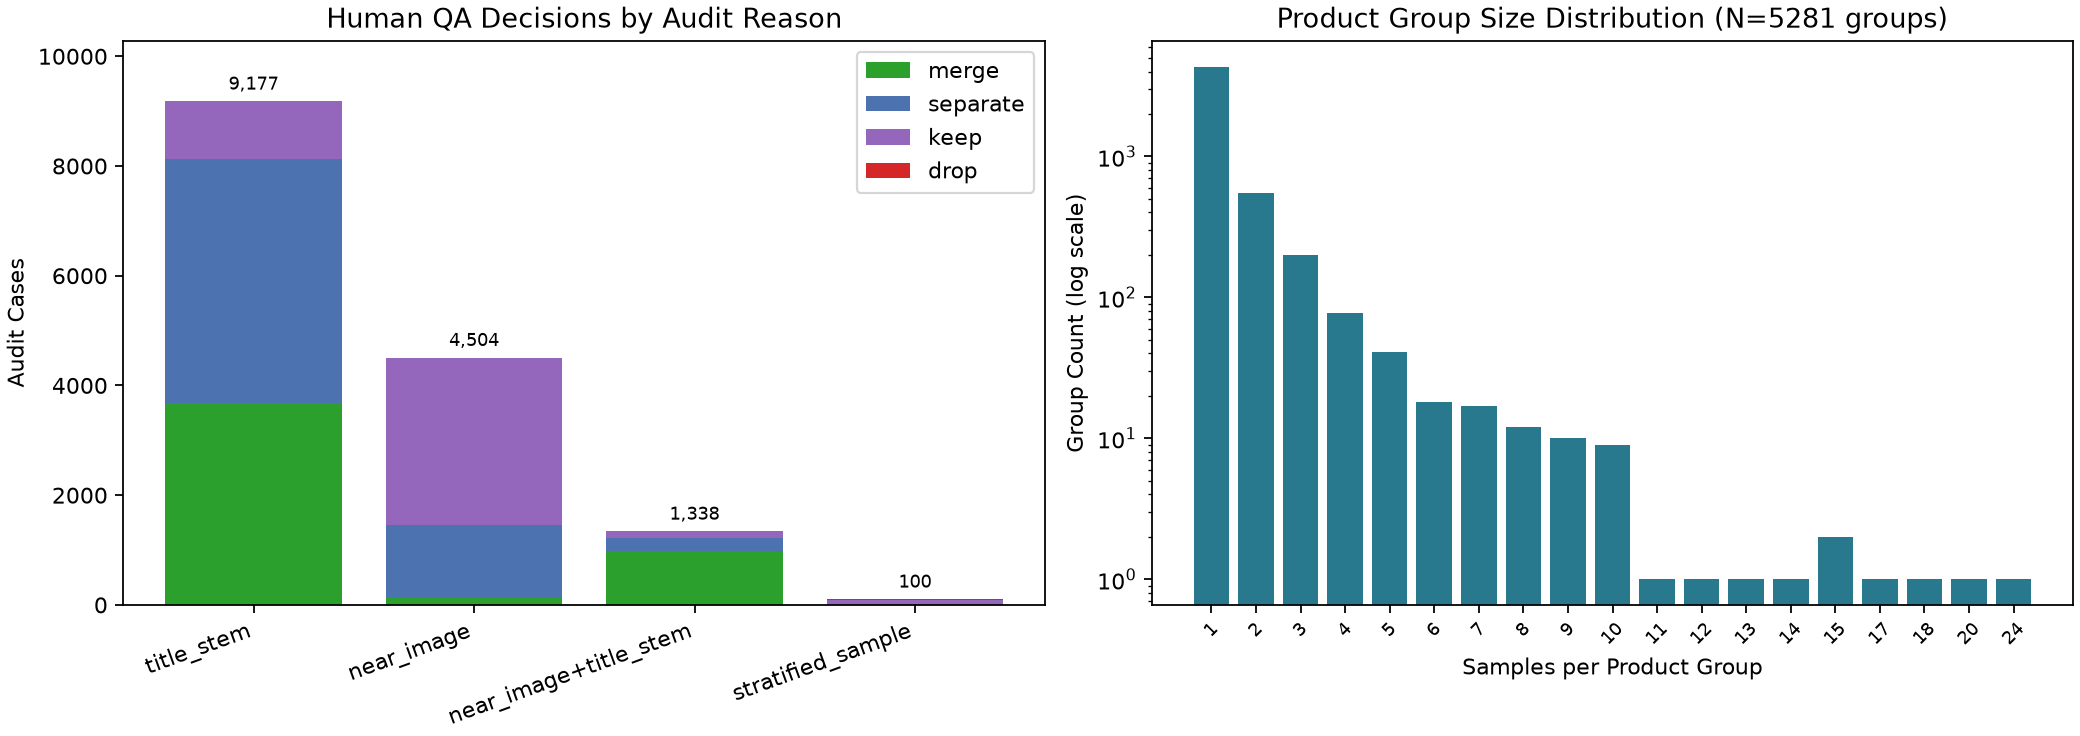
\includegraphics[width=.91\linewidth]{assets/eda/curation_and_groups.png}
\caption{Review decisions by audit reason and reviewed group sizes. The right panel uses a logarithmic frequency axis. Source: saved cohort EDA~[8].}
\label{fig:eda-curation}
\end{figure}

Figure~\ref{fig:eda-curation} shows 4,333 singletons and 948 multi-listing groups, with up to 24 items per group. After screening, no listing lacks a title or readable photo, and zero decoded-image hashes repeat.

\clearpage
\subsection{Class balance and group isolation}
The splitter targets 70/15/15 per class at seed 36, assigning whole groups. Table~\ref{tab:split} lists 5,052 training, 1,083 validation and 1,081 test listings. The 5,281 product groups divide into 3,310 train, 981 validation and 990 test groups. A direct check finds zero groups shared across splits and zero groups containing multiple catalog labels.

\begin{table}[H]
\centering
\small
\caption{Frozen membership by catalog class. Counts refer to paired listings.}
\label{tab:split}
\begin{tabular}{@{}lrrrr@{}}
\toprule
Class & Train & Validation & Test & Total\\ \midrule
\ABOSplitRows
\midrule
All classes & 5,052 & 1,083 & 1,081 & 7,216\\
\bottomrule
\end{tabular}
\end{table}

\begin{figure}[H]
\centering
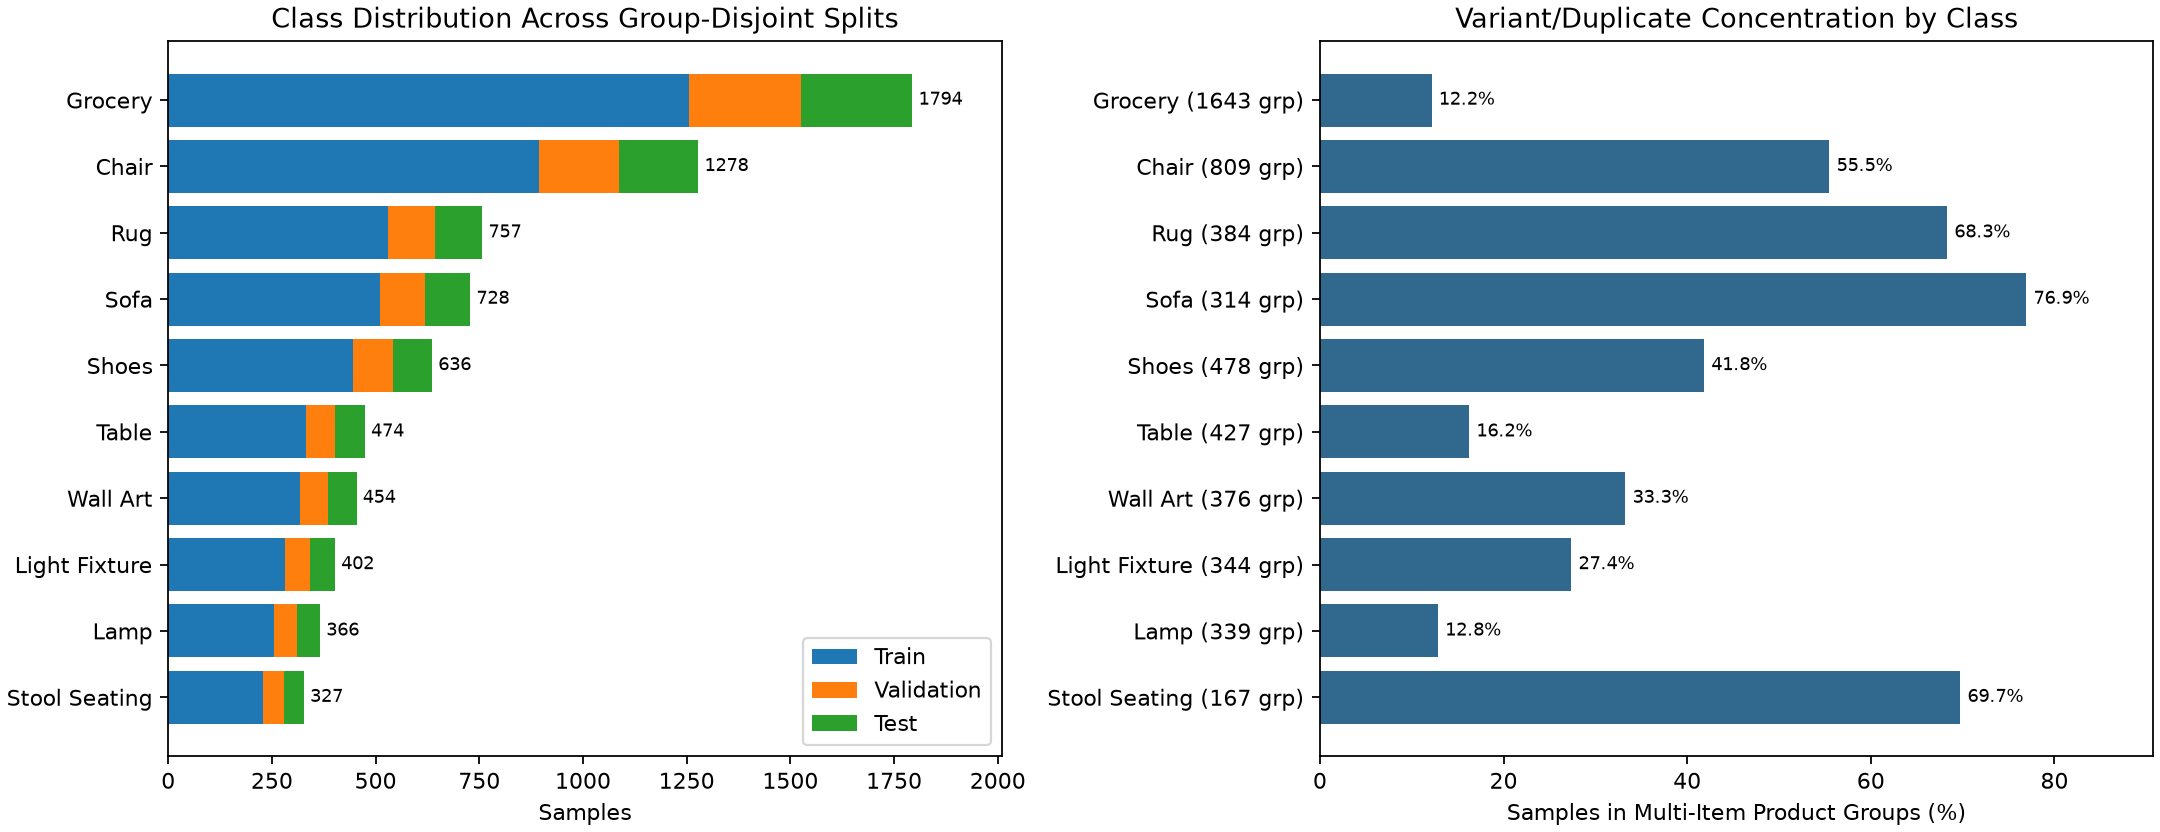
\includegraphics[width=.92\linewidth]{assets/eda/split_and_class_distribution.png}
\caption{Left: class counts by split. Right: fraction of each class in groups with multiple listings. Source: saved cohort EDA~[8].}
\label{fig:eda-split}
\end{figure}

Across the cohort, GROCERY has 1,794 listings and STOOL\_SEATING has 327, a \(5.49{:}1\) imbalance. On test they contribute 269 and 49 listings respectively. We report macro-F1 alongside accuracy so each class has equal weight in the primary metric. Multi-item groups cover 76.9\% of SOFA listings and 69.7\% of STOOL\_SEATING listings, compared with 12.2\% for GROCERY.

\clearpage
\subsection{Title length and class-name masking}
Before subword tokenization, titles contain a median of 13 whitespace-separated words, with quartiles of 10 and 16, a 95th percentile of 21 and a range of 1 to 34. The median title is 77 characters long. Table~\ref{tab:eda-title-split} tracks the small change in length between splits and the coverage of the fixed mask.

\begin{table}[H]
\centering
\small
\caption{Title length and fixed-lexicon masking by split. Percentages use the listing count in each row.}
\label{tab:eda-title-split}
\begin{tabular}{@{}lrrrr@{}}
\toprule
Split & Titles & Median words & Changed by mask & Changed (\%)\\ \midrule
Train & 5,052 & 13 & 2,365 & 46.8\\
Validation & 1,083 & 12 & 493 & 45.5\\
Test & 1,081 & 12 & 479 & 44.3\\
\midrule
All splits & 7,216 & 13 & 3,337 & 46.2\\
\bottomrule
\end{tabular}
\end{table}

\begin{figure}[H]
\centering
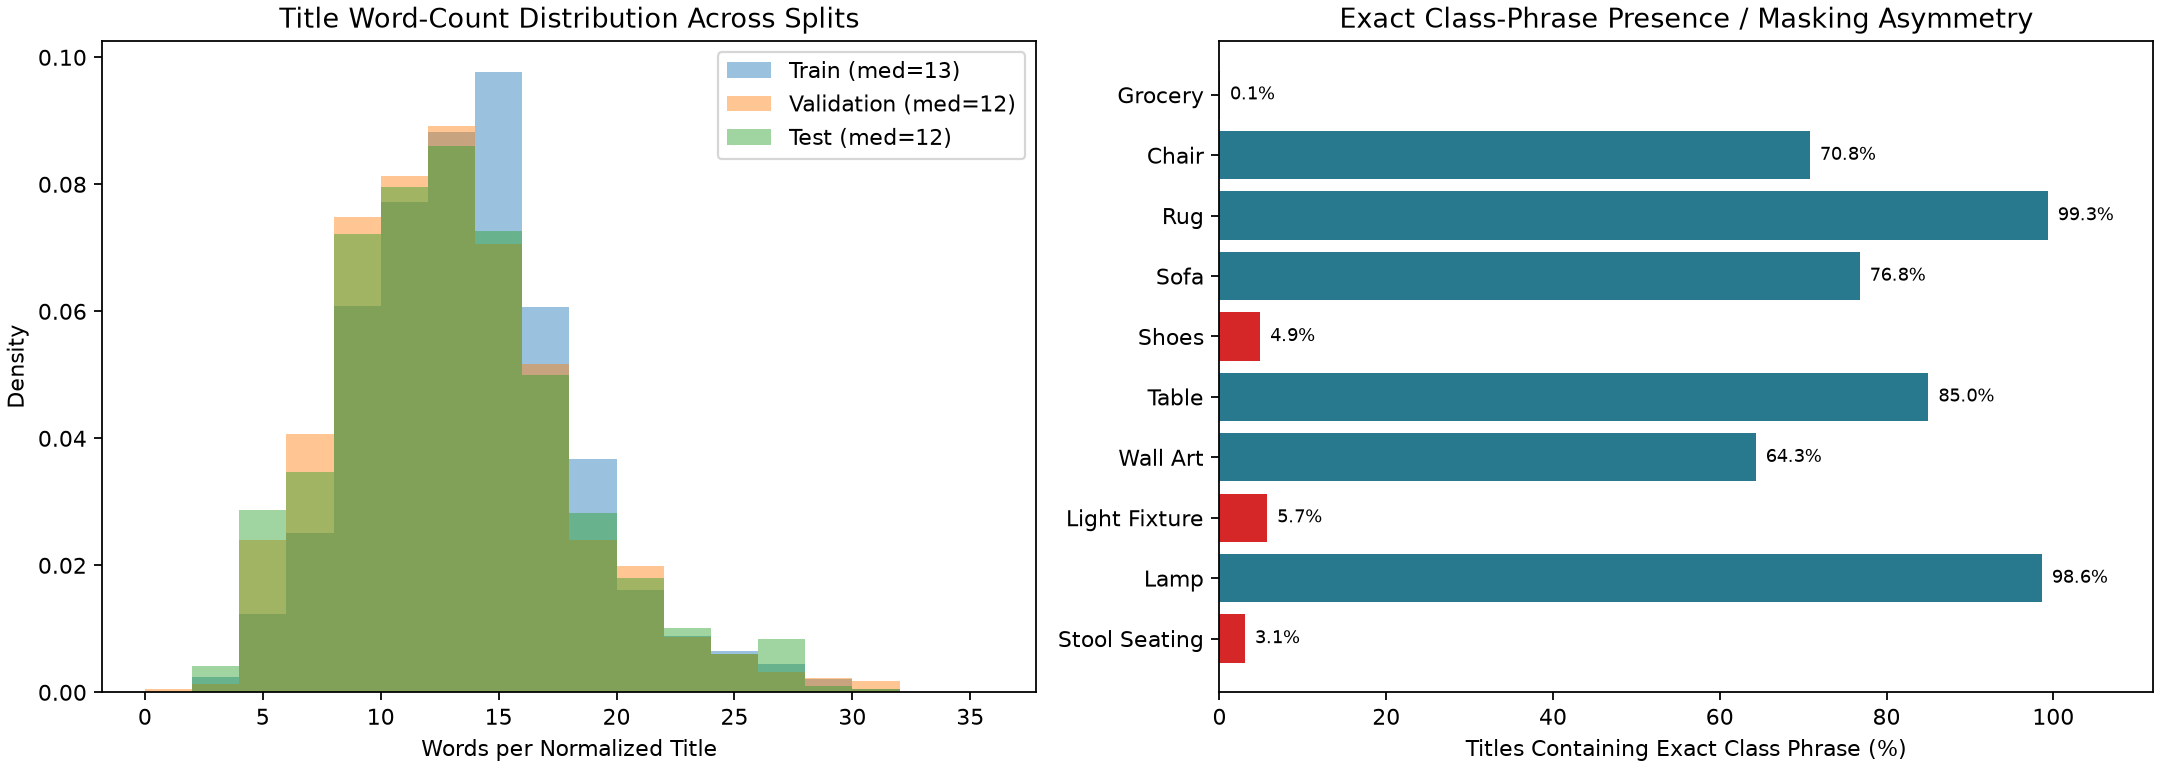
\includegraphics[width=.98\linewidth]{assets/eda/title_length_and_masking.png}
\caption{Original title length and the fraction of titles changed by an exact match to any phrase in the common class-name lexicon. The right panel groups listings by their true catalog label. Source: saved cohort EDA~[8].}
\label{fig:eda-titles}
\end{figure}

The class-name mask affects 99.3\% of RUG titles, 98.6\% of LAMP titles and 85.0\% of TABLE titles. It affects 0.1\% of GROCERY titles and 3.1\% of STOOL\_SEATING titles. A single global rule removes explicit names unevenly. For example, STOOL\_SEATING can retain related terms such as \emph{stool} and \emph{bar} when the exact phrase does not occur. This difference matters when interpreting the title baseline under the fixed policy.

\clearpage
\subsection{Photo geometry and visual context}
The JPEGs are capped at 256 pixels on the longest side. Their median width and height are both 256 pixels. The minimum width is 54 pixels and the minimum height is 36 pixels. Of the 7,216 images, 7,188 are originally RGB and 28 are grayscale. The image adapter converts all of them to RGB before resizing.

We flag a photo as extreme when its width-to-height ratio is below 0.5 or above 2.0. There are 767 such images (10.6\%). For a short-edge resize to 256 and a \(224\times224\) center crop, the retained area fraction is approximated by \((224/256)^2\min(w,h)/\max(w,h)\) for source dimensions \(w,h\). The cohort mean is 62.8\%. GROCERY and SHOES have extreme ratios on 27.0\% and 26.7\% of images respectively, with mean crop-retention estimates of 49.1\% and 50.3\%.

\begin{figure}[H]
\centering
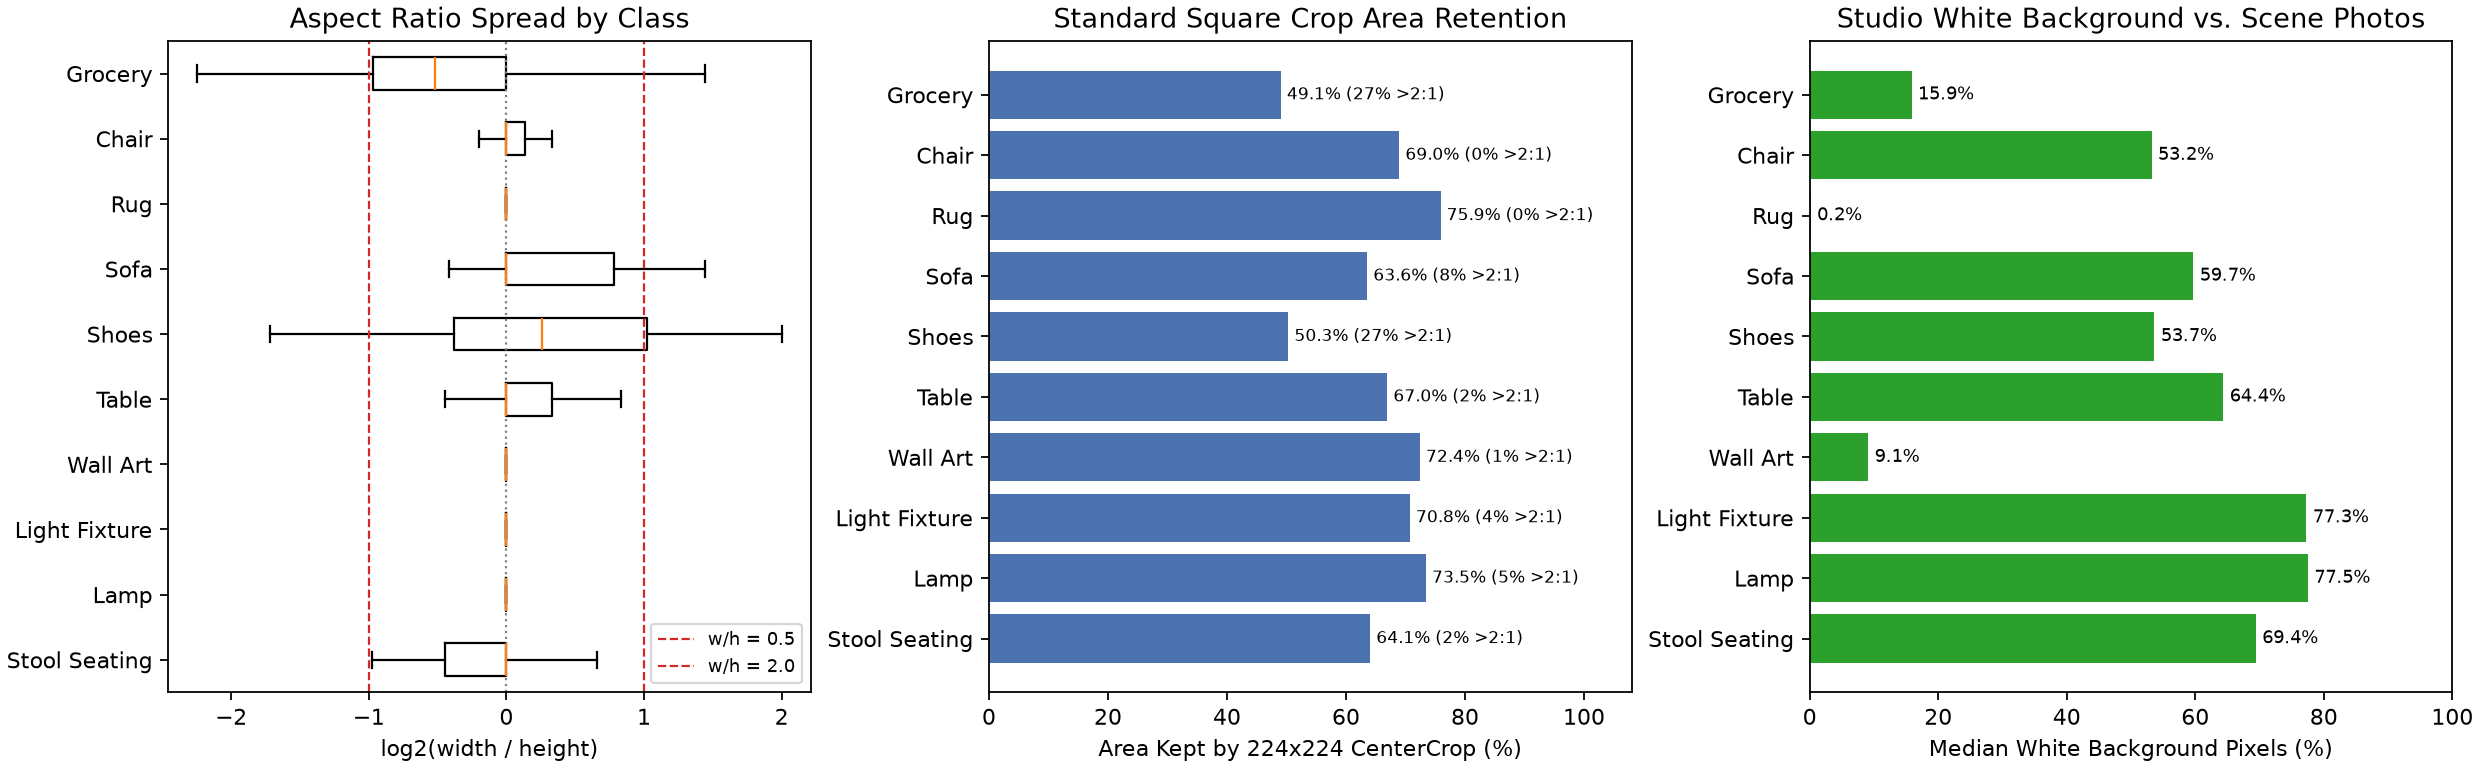
\includegraphics[width=.98\linewidth]{assets/eda/image_geometry_and_background.png}
\caption{Image aspect ratio, estimated area retained after the center crop and median near-white pixel share by class. Near-white means all three RGB channels are at least 245. Source: saved cohort EDA~[8].}
\label{fig:eda-image}
\end{figure}

The median near-white share is 77.5\% for LAMP and 77.3\% for LIGHT\_FIXTURE, compared with 0.2\% for RUG and 9.1\% for WALL\_ART. Near-white share can reflect the object itself or the image background. The geometry and pixel-space differences identify potential visual cues and show where cropping can remove substantial context. The experiment uses the same image transform for each image-based model.

\clearpage
\subsection{Repeated titles and cross-modal ambiguity}
Unicode normalization, whitespace collapse and case folding leave 106 title strings that recur across 241 listings. Of these strings, 66 occur in more than one reviewed group, 43 occur across splits, and 9 are shared by multiple catalog labels. The nine cross-label strings cover 26 listings. Group isolation preserves the reviewed product boundary while allowing titles to repeat for different items.

\begin{figure}[H]
\centering
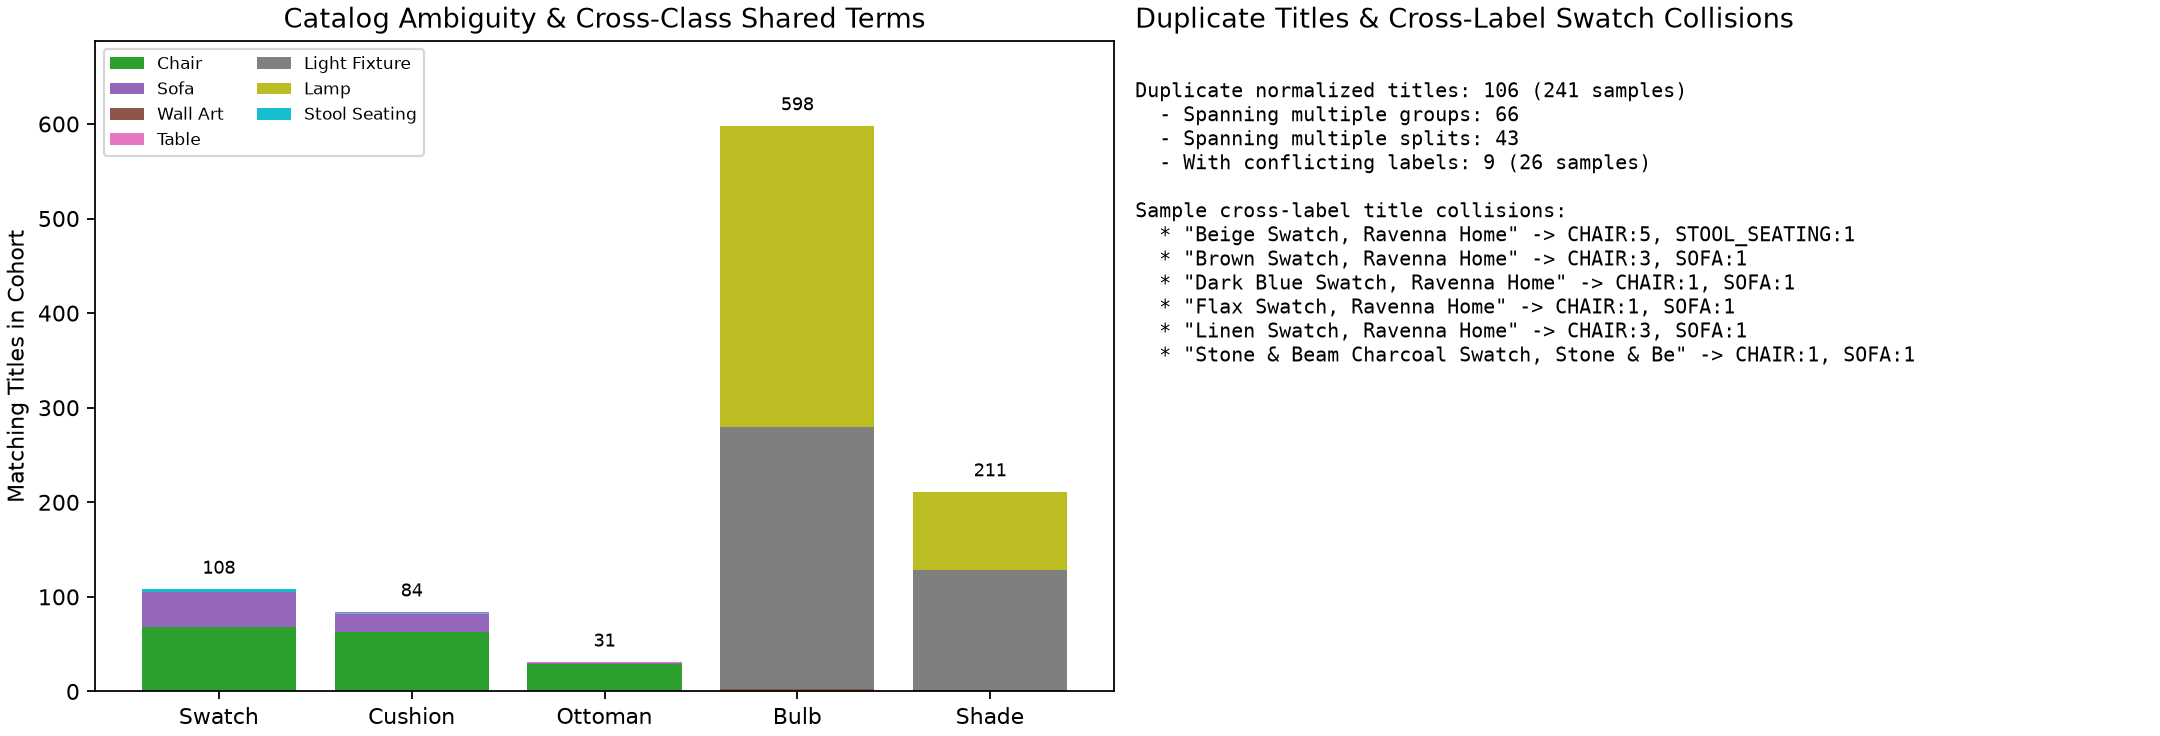
\includegraphics[width=.98\linewidth]{assets/eda/multimodal_ambiguity_and_noise.png}
\caption{Frequency of selected ambiguity terms and examples of repeated titles with different catalog labels. Counts match a term or its plural in the title. Source: saved cohort EDA~[8].}
\label{fig:eda-ambiguity}
\end{figure}

Among the seating labels, 108 listings mention \emph{swatch}, including 68 CHAIR and 37 SOFA listings. Across the cohort, \emph{bulb} appears in 598 titles, including 318 LAMP and 277 LIGHT\_FIXTURE listings. Both terms span several classes and can be ambiguous without more context.

\newcommand{\edapair}[3]{%
\begin{minipage}[t]{.153\linewidth}
\centering
\includegraphics[width=.96\linewidth,height=25mm,keepaspectratio]{assets/eda/#1.jpg}\par
{\scriptsize\textbf{#2}\par #3\par\code{#1}}
\end{minipage}}
\begin{figure}[H]
\centering
\edapair{B074MFTWGX}{Grocery}{Coconut water}\hfill
\edapair{B07Q2R4FBS}{Shoes}{Chukka boots}\hfill
\edapair{B07QF91L1T}{Lamp}{Table lamp}\hfill
\edapair{B07QGHVVHG}{Light fixture}{Flush mount}\hfill
\edapair{B07KR2S2DW}{Chair}{Dark blue swatch}\hfill
\edapair{B07KR8HR2F}{Sofa}{Dark blue swatch}
\caption{Six frozen training pairs, with shortened titles. The last two share the full title \emph{Dark Blue Swatch, Ravenna Home} and show fabric samples under different catalog labels. Photos from Amazon Berkeley Objects, CC BY 4.0~[1].}
\label{fig:eda-gallery}
\end{figure}

The gallery contrasts useful agreement, such as the chukka boot image and title, with paired swatches that show and describe fabric. The seating type is difficult to recover from the latter pair because neither input depicts the catalog object.

\clearpage
\subsection{Residual cues in training titles}
We inspected brand metadata and residual terms on the training split. Of 5,052 training listings, 5,051 have a recorded brand across 76 distinct brand strings. A brand's dominant-class share is the fraction of its listings assigned to its most common class. Table~\ref{tab:eda-brands} contrasts broad furniture brands with brands whose sampled products concentrate in one class.

\begin{table}[H]
\centering
\small
\caption{Selected brand--label associations measured on train only.}
\label{tab:eda-brands}
\begin{tabular}{@{}lrrlr@{}}
\toprule
Brand & Listings & Classes & Dominant class & Share\\ \midrule
Stone \& Beam & 1,253 & 8 & CHAIR & 26.6\%\\
Rivet & 1,231 & 8 & CHAIR & 21.2\%\\
365 by Whole Foods Market & 427 & 1 & GROCERY & 100.0\%\\
find. & 198 & 1 & SHOES & 100.0\%\\
\bottomrule
\end{tabular}
\end{table}

\begin{figure}[H]
\centering
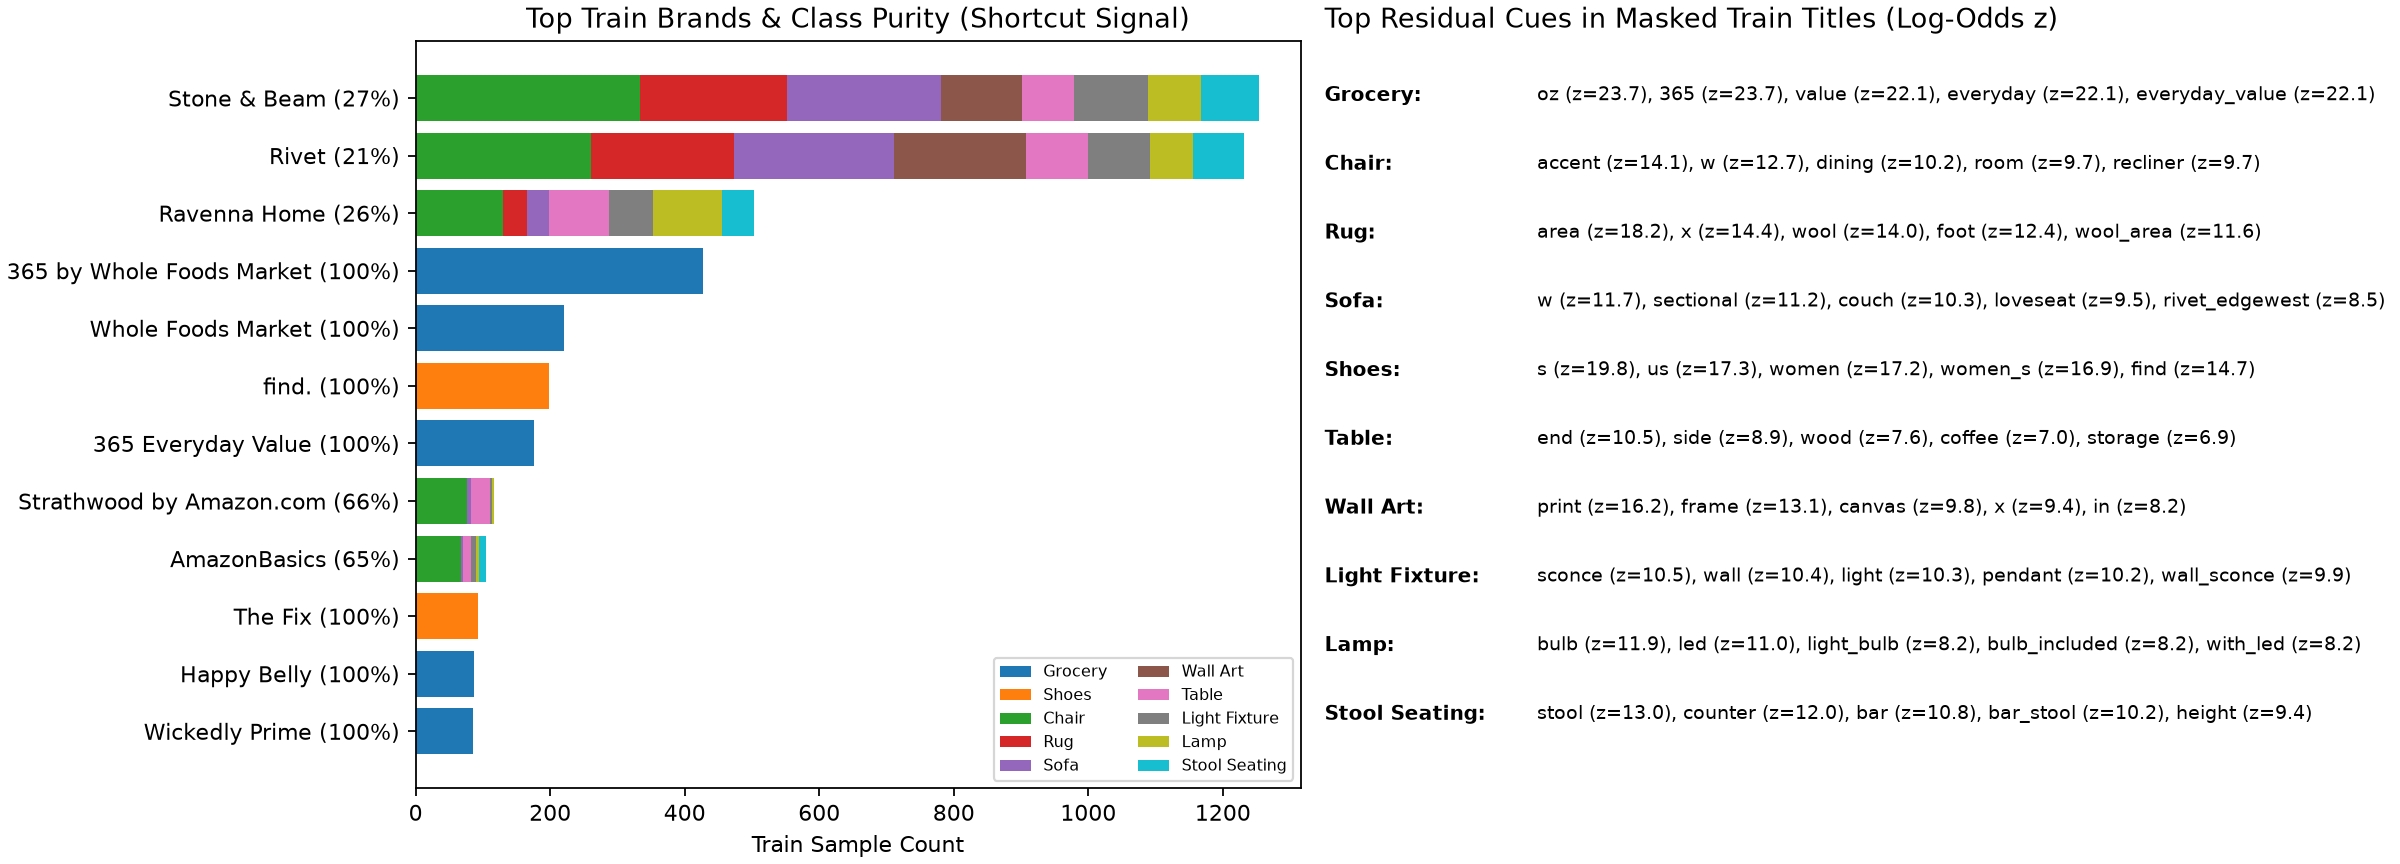
\includegraphics[width=.98\linewidth]{assets/eda/train_brand_and_lexical_cues.png}
\caption{Brand composition and residual word and phrase associations in masked training titles. The latter are ranked by smoothed log-odds relative to the other classes. Source: saved cohort EDA~[8].}
\label{fig:eda-lexical}
\end{figure}

After masking, \code{oz} occurs in 638 training titles and \code{365} in 636, all in GROCERY. \code{sconce} occurs in 109 training titles, 107 with label LIGHT\_FIXTURE. The model receives the title string, which can contain brand names or related terms. The separate brand metadata field is used in this diagnostic. These observations document associations that remain after masking and should be considered when assessing generalization to other catalogs.



\clearpage
\section{Methodology}
\subsection{Pipeline overview}
A full encoder batch has 32 aligned listings. The image tensor is \([32,3,224,224]\), and the token IDs and attention masks are \([32,L]\) with \(L\leq64\). Training reads up to 128 paired feature rows and their integer class labels per batch using the manifest IDs.

\begin{figure}[H]
\centering
\small
\stage{Listing ID, image, title and label}
\(\longrightarrow\)
\stage{Group split and input preparation}\\[0.65em]
\stage{Frozen ResNet-18 / frozen DistilBERT}
\(\longrightarrow\)
\stage{Aligned feature caches}\\[0.65em]
\stage{Projection and fusion}
\(\longrightarrow\)
\stage{Head logits and cross-entropy}
\(\longrightarrow\)
\stage{Validation and test}
\caption{Two encoders produce feature rows indexed by listing ID. Head training uses cross-entropy, validation selects checkpoints, and the locked suite supplies the held-out predictions.}
\end{figure}

\subsection{Image modality}
The image branch corrects EXIF orientation, converts the photo to RGB and applies the resize, center crop and normalization supplied with the torchvision ImageNet-1K V1 weights. ResNet-18 runs in evaluation mode with its classification layer removed, producing a 512-dimensional frozen feature for each listing~[3]. The benchmark uses no stochastic image augmentation.

\subsubsection{Image input and representation EDA}
Table~\ref{tab:mod-image} uses the crop-area estimate from Section~\ref{sec:eda} and the original image cache~[9]. It compares how much of the resized frame is retained and the Euclidean norm of the resulting feature vector. A low-area flag means the crop retains less than half of the resized frame.

\begin{table}[H]
\centering
\small
\caption{Image-only EDA by split. Norm is the median \(\ell_2\) feature norm with interquartile range in brackets.}
\label{tab:mod-image}
\begin{tabular}{@{}lrrr@{}}
\toprule
Split & Median area retained & Low-area images & Feature norm [Q1, Q3]\\ \midrule
Train & 72.1\% & 1,244 (24.6\%) & 26.75 [24.24, 29.44]\\
Validation & 73.9\% & 257 (23.7\%) & 26.58 [23.67, 29.35]\\
Test & 70.9\% & 256 (23.7\%) & 26.49 [23.93, 29.27]\\
All splits & 72.4\% & 1,757 (24.3\%) & 26.70 [24.11, 29.41]\\
\bottomrule
\end{tabular}
\end{table}

The 256 low-area test images provide cases for checking whether the item survives cropping. Median image-feature norms range from 26.49 to 26.75 across splits.


\clearpage
\subsection{Title modality}
\label{sec:preprocess}
The title branch normalizes Unicode to NFKC and collapses whitespace. It replaces matches to the common lexicon of class names with \code{[MASK]}, regardless of the listing's true label. The benchmark uses no optional extra phrases. DistilBERT Base Uncased is frozen at revision \code{12040accade4e8a0f71eabdb258fecc2e7e948be} using Hugging Face Transformers 4.57.6. The branch takes the 768-dimensional first-token state as its feature~[4]. The tokenizer uses dynamic batch padding and a 64-token cap.

\subsubsection{Title input and representation EDA}
We ran the pinned tokenizer on the normalized, masked titles before truncation or padding, with special tokens included~[9]. Table~\ref{tab:mod-title} measures subword sequence lengths under the benchmark's tokenizer.

\begin{table}[H]
\centering
\small
\caption{Title-only EDA by split. P95 is the upper empirical 95th percentile of unpadded sequence length.}
\label{tab:mod-title}
\begin{tabular}{@{}lrrrrr@{}}
\toprule
Split & Median tokens & P95 & Max. tokens & Above 64 & Median feature norm\\ \midrule
Train & 22 & 31 & 53 & 0 & 11.97\\
Validation & 21 & 32 & 46 & 0 & 11.99\\
Test & 21 & 31 & 45 & 0 & 11.99\\
All splits & 22 & 31 & 53 & 0 & 11.98\\
\bottomrule
\end{tabular}
\end{table}

The longest sequence has 53 tokens, so all 7,216 masked titles fit within the 64-token limit. Masking changes what some terms convey even when their token sequences fit under the cap.


\subsection{Paired modalities and fusion}
\subsubsection{Alignment and joint input EDA}
The two caches each contain one finite, nonzero feature vector for every one of the 7,216 manifest IDs, in the same order~[9]. This gives 5,052 training, 1,083 validation and 1,081 test pairs with both modalities available. Each fusion condition uses these same pairs and the catalog label as its target.

Table~\ref{tab:mod-paired} crosses the image low-area flag with whether the title's class-name mask changed at least one phrase. The columns are disjoint and sum to the paired membership in each split. For example, an image crop can remove a large part of the frame while the title still retains its original words.

\begin{table}[H]
\centering
\small
\caption{Paired input EDA. Low area means less than 50\% estimated frame retention. Mask means the title changed under the fixed rule.}
\label{tab:mod-paired}
\begin{tabular}{@{}lrrrr@{}}
\toprule
Split & Neither flag & Low area only & Mask only & Both flags\\ \midrule
Train & 1,686 & 1,001 & 2,122 & 243\\
Validation & 385 & 205 & 441 & 52\\
Test & 398 & 204 & 427 & 52\\
All splits & 2,469 & 1,410 & 2,990 & 347\\
\bottomrule
\end{tabular}
\end{table}

Both flags occur in 52 test listings (4.8\%). The combination varies by class. Among all SOFA listings, 200 of 728 have both flags. In GROCERY, 975 of 1,794 trigger the low-area flag, while only 1 title changes under the mask. These flags describe the observed inputs. The benchmark results assess prediction performance separately.

\subsubsection{Fusion heads and objective}
For each input modality, we learn a linear projection and ReLU activation. Let \(u=\operatorname{ReLU}(W_i f_i+b_i)\) and \(v=\operatorname{ReLU}(W_t f_t+b_t)\), with \(u,v\in\mathbb{R}^{128}\). We compare the intermediate representations below. Every representation feeds a 128-wide ReLU hidden layer and a ten-logit output layer.

\begin{table}[H]
\centering
\caption{Fusion inputs at the head interface.}
\begin{tabularx}{\linewidth}{@{}p{.24\linewidth}p{.23\linewidth}Y@{}}
\toprule
Condition & Input to the head & Design role\\ \midrule
Image-only & \(u\) & Measures discriminative signal in the photograph.\\
Title-only & \(v\) & Measures signal in the masked title.\\
Concat & \([u;v]\) & Combines the two representations directly.\\
\bottomrule
\end{tabularx}
\end{table}

We minimize unweighted multiclass cross-entropy \(-\log p_\theta(y\mid I,T)\) over each training batch. The unimodal versions apply the same objective to one input. There are no auxiliary per-branch losses. Concat requires both cached feature rows.

\subsection{Training and evaluation protocol}
Each run uses AdamW, a learning rate of \(10^{-3}\), batch size 128, and eight epochs. There is no learning-rate scheduler or early stopping. Runs use the same 128-dimensional projection, split, encoder settings, loss and optimizer budget. Each model is trained once with each seed in \(\{69420,67,69\}\). The checkpoint with highest validation macro-F1 is retained, with ties favoring the earlier epoch. The suite fixes these checkpoints before held-out scoring.

Macro-F1 is the arithmetic mean of the ten class F1 scores. Each class F1 is the harmonic mean of precision and recall. Accuracy is the fraction of test listings correctly classified. We report the mean and sample standard deviation across the three seeds. All reported seed comparisons hold the test membership fixed.

\subsection{Comparison design}
We test whether adding the title to image-based recognition improves classification. The two single-input heads establish how much information each modality carries on its own. Concat uses both 128-dimensional projections, so its input layer is wider. The comparison evaluates the complete simple-fusion design under a common split, encoder policy, training budget, checkpoint criterion and matched seeds.

The unimodal reference is selected using mean validation macro-F1 across the three seeds. The primary comparison is the paired test macro-F1 difference between concat and that reference. A positive difference at the same seed favors concat on this cohort. Accuracy and class-level F1 provide context for the aggregate comparison.

\section{Draft benchmark results}
\subsection{Aggregate results and paired differences}
Table~\ref{tab:main} summarizes nine runs, with three seeds for each configuration. Image-only is the validation-selected unimodal reference. Concat gives the highest mean held-out macro-F1 and accuracy among the three M2 configurations.

\begin{table}[H]
\centering
\small
\caption{Validation and test results in percent, reported as mean \(\pm\) sample SD across three seeds.}
\label{tab:main}
\begin{tabular}{@{}lrrr@{}}
\toprule
Model & Validation macro-F1 & Test macro-F1 & Test accuracy\\ \midrule
\ABOMainRows
\bottomrule
\end{tabular}
\end{table}

\begin{table}[H]
\centering
\small
\caption{Held-out macro-F1 difference in percentage points for the same seed.}
\label{tab:deltas}
\begin{tabular}{@{}lrrrrr@{}}
\toprule
Pair & 69420 & 67 & 69 & Mean & SD\\ \midrule
\ABODeltaRows
\bottomrule
\end{tabular}
\end{table}

Concat improves over the stronger unimodal reference at every seed (Table~\ref{tab:deltas}). The mean difference is 3.69 points, with a sample SD of 0.13 points. These seeds vary optimization on one fixed split, so the sample SD describes run variation on that split.

\subsection{Checkpoints and class performance}
All nine runs completed eight epochs. Table~\ref{tab:seeds} shows the selected epoch for each score. Validation selected epoch 7 or 8 in every run, including epoch 7 for concat at seeds 69420 and 67.

\begin{table}[H]
\centering
\small
\caption{Test macro-F1 (\%) with the best validation epoch in parentheses.}
\label{tab:seeds}
\begin{tabular}{@{}lrrr@{}}
\toprule
Model & 69420 & 67 & 69\\ \midrule
\ABOSeedRows
\bottomrule
\end{tabular}
\end{table}

Table~\ref{tab:class} shows where fusion helps most. For LAMP, concat reaches 95.79\% class F1, versus 88.01\% for image-only and 89.78\% for title-only. WALL\_ART shows the opposite pattern. Title-only reaches 98.09\%, ahead of concat at 95.71\%.

\begin{table}[H]
\centering
\small
\caption{Held-out class support and mean F1 (\%) across the same three seeds.}
\label{tab:class}
\begin{tabular}{@{}lrrrr@{}}
\toprule
Class & Test support & Image-only & Title-only & Concat\\ \midrule
\ABOClassRows
\bottomrule
\end{tabular}
\end{table}

\subsection{Matched examples}
The following examples use the same test listings and seed 69420. The images and catalog labels are from the frozen cohort. The examples refer to the original titles. The title model uses the masked inputs described in Section~\ref{sec:preprocess}.

\newcommand{\caseblock}[4]{%
\begin{minipage}[c]{.20\linewidth}\centering\includegraphics[width=.94\linewidth,height=25mm,keepaspectratio]{assets/#1.jpg}\end{minipage}\hfill
\begin{minipage}[c]{.76\linewidth}
\raggedright
\textbf{#2}\quad\code{#1}\par
{\small #3\par #4}
\end{minipage}\par\vspace{0.55em}
}

\caseblock{B075X4WBLM}{Concat recovers the catalog label}
{The title describes an armless settee, with a photograph of a compact upholstered seat.}
{Label SOFA. Image-only and title-only predict CHAIR, while concat predicts SOFA.}

\caseblock{B001BQAMNW}{The title-only cue is stronger in this example}
{The title describes vinyl dining chairs. The photograph shows one seat with a boxy frame.}
{Label CHAIR. Title-only predicts CHAIR. Image-only and concat predict TABLE.}

\caseblock{B075YMY2J7}{Concat fails despite two correct unimodal predictions}
{The title describes an accent-chair set, and the photograph shows two upholstered seats.}
{Label CHAIR. Both single-input models predict CHAIR. Concat predicts STOOL\_SEATING.}

{\footnotesize Catalog photographs from Amazon Berkeley Objects, CC BY 4.0, resized for display~[1].}

The examples show that better aggregate scores can coexist with individual failures. Across the three seeds, concat corrected 132 image-only mistakes and introduced 44 errors on listings previously classified correctly. These are counts of seed--listing decisions on repeated test membership~[5].

\section{Compute, reproducibility and limitations}
\subsection{Measured compute}
The frozen image encoder took 384.41 seconds for 7,216 images and the frozen title encoder took 297.02 seconds for 7,216 titles. These are separate Windows AMD64 CPU measurements at encoder batch size 32 with PyTorch 2.13.0+cpu. They include batch preprocessing, forward passes and transfers. They exclude model download and initialization. The two cached feature matrices contain approximately 35.23 MiB of float32 values before IDs, metadata and archive overhead.

The collected head runs used Tesla T4 GPUs, Linux x86-64, PyTorch 2.14.1+cu130 and CUDA 13.0. The fit-loop ranges in Table~\ref{tab:compute} include training and validation for eight epochs, excluding feature extraction, notebook setup and artifact writes. The held-out scorer ran on CPU and includes batching, transfers, loss and metric computation from cached vectors. Its receipts do not specify a CPU model. These short scoring times are useful for describing this notebook workload. End-to-end latency for a fresh image--title pair requires encoder inference and a separate measurement.

\begin{table}[H]
\centering
\small
\caption{Trainable head size and observed compute scopes. Cached test time covers the full 1,081-listing split and is reported as mean \(\pm\) sample SD.}
\label{tab:compute}
\begin{tabular}{@{}lrrr@{}}
\toprule
Model & Head parameters & T4 fit range (s) & CPU cached test (ms)\\ \midrule
\ABOComputeRows
\bottomrule
\end{tabular}
\end{table}

\subsection{Reproduce the comparison}
Use the team's \code{abo-v1} manifest, exact source ZIP and two frozen feature caches~[5,6]. In the archived \code{abo-v1-main} suite, read the nine validation-selected checkpoints and their test rows for image-only, title-only and concat. Use the four notebooks in order to prepare the cohort, train and collect the suite, score the selected checkpoints and regenerate its analysis. The reported rows use manifest identity \path{9742854841e0b0d1afe752dc080a990707b47ba82a109a0180b5abb90a158d1a}.

\subsection{Limitations and conclusion}
The results cover one marketplace, ten catalog classes and one group-disjoint split, with variation measured over three optimization seeds. The title mask leaves synonyms and other wording, and changes different shares of titles in each class. Concat uses both feature rows in this evaluation.

Simple concatenation improves mean macro-F1 by 3.69 points over the stronger unimodal baseline on this cohort. The class results and matched examples identify cases where fusion adds useful context and cases where a single modality remains more reliable.

\clearpage
\section{Team work and AI usage}
The team's A3 allocation assigns dataset and image work to \vn{Nguyễn Hạo Thiên}, title and evaluation work to \vn{Nguyễn Anh Khoa}, and fusion and integration to \vn{Tạ Tuấn Khải}. This describes the planned division of work. \vn{Tạ Tuấn Khải} provided curation decisions and coordinated the official notebook workflow. The team should confirm individual contributions before submission.

OpenAI Codex assisted with planning, code, tests, notebook orchestration, rule-based curation, results verification and drafting this report. The quantitative results come from the locked benchmark, per-run checkpoints and held-out predictions. The report uses aggregate analysis artifacts and verified matched examples. The repository's A3 disclosure records the scope of assistance~[6].

\begin{samepage}
\section*{References and experiment artifacts}
\phantomsection
\addcontentsline{toc}{section}{References and experiment artifacts}
\begin{enumerate}
\item Amazon and UC Berkeley. \source{https://amazon-berkeley-objects.s3.us-east-1.amazonaws.com/index.html}{Amazon Berkeley Objects dataset release, download and attribution}. Dataset license: CC BY 4.0.
\item Collins et al. \source{https://openaccess.thecvf.com/content/CVPR2022/html/Collins_ABO_Dataset_and_Benchmarks_for_Real-World_3D_Object_Understanding_CVPR_2022_paper.html}{ABO: Dataset and Benchmarks for Real-World 3D Object Understanding}. CVPR, 2022.
\item He et al. \source{https://openaccess.thecvf.com/content_cvpr_2016/html/He_Deep_Residual_Learning_CVPR_2016_paper.html}{Deep Residual Learning for Image Recognition}. CVPR, 2016. See the \source{https://docs.pytorch.org/vision/stable/models/generated/torchvision.models.resnet18.html}{torchvision ResNet-18 weights and transforms}.
\item Sanh et al. \source{https://arxiv.org/abs/1910.01108}{DistilBERT, a distilled version of BERT}. 2019. See the \source{https://huggingface.co/distilbert/distilbert-base-uncased}{model and tokenizer}.
\item Tiki-taka. \source{https://drive.google.com/drive/folders/1UMayAvNgLG3IM5x_C7dVYo_VJc8kcZi0}{Official suite} and \source{https://drive.google.com/drive/folders/1Sa2vh_SJiCH8ZsHjvW9fLZdYda61oKzm}{analysis outputs}, verified 22 November 2026. The analysis folder contains aggregate scores, class-level scores, agreement categories and matched errors. Access follows team Drive permissions.
\item Tiki-taka. \source{https://github.com/TuanKhai1210/Deep-Learning-Benchmark-Suite/tree/feat/a3-basecode/configs/a3}{A3 source and reproduction guide} and \source{https://github.com/TuanKhai1210/Deep-Learning-Benchmark-Suite/blob/feat/a3-basecode/docs/a3-ai-usage.md}{A3 AI usage disclosure}.
\item CO3133 Course Project Handbook v2, 14 September 2026, Sections 3--4, 7.6 and 25--32.
\item Tiki-taka. Dataset EDA for the frozen \code{abo-v1} cohort, \path{runs/a3/eda-abo-v1/eda_summary.json} and \code{notebooks/a3_eda.ipynb} in the team archive. Read back and independently checked against the manifest, review decisions and image inventory on 23 November 2026.
\item Tiki-taka. Modality input audit, verified on 23 November 2026 from the frozen cohort, locked feature caches and pinned tokenizer. Aggregate counts are packaged as \path{assets/modality-eda.json}.
\end{enumerate}
\end{samepage}
\end{document}
